
\documentclass{beamer}

\mode<presentation>
{
  \usetheme{Boadilla}
  \setbeamercovered{transparent}
}


\usepackage{cmap}					% поиск в PDF
\usepackage[T2A]{fontenc}			% кодировка
\usepackage[utf8]{inputenc}			% кодировка исходного текста
\usepackage[russian, english]{babel}	% локализация и переносы
\usepackage{mathtext}
\usepackage{times}
\usepackage{subfigure}
\usepackage{caption}
\usepackage{wrapfig}


%Листинг
\usepackage{listings}
\usepackage{color}
 
\definecolor{codegreen}{rgb}{0,0.6,0}
\definecolor{codegray}{rgb}{0.5,0.5,0.5}
\definecolor{codepurple}{rgb}{0.58,0,0.82}
\definecolor{backcolour}{rgb}{0.95,0.95,0.92}
 
\lstdefinestyle{mystyle}{
    backgroundcolor=\color{backcolour},   
    commentstyle=\color{codegreen},
    keywordstyle=\color{magenta},
    numberstyle=\tiny\color{codegray},
    stringstyle=\color{codepurple},
    basicstyle=\footnotesize,
    breakatwhitespace=false,         
    breaklines=true,                 
    captionpos=b,                    
    keepspaces=true,                 
    numbers=left,                    
    numbersep=5pt,                  
    showspaces=false,                
    showstringspaces=false,
    showtabs=false,                  
    tabsize=2
}
\lstset{style=mystyle}
 
% title
\title[дисперсия] % (optional, use only with long paper titles)
{reflectance}



\institute[] % (optional, but mostly needed)


\date[\today ] % (optional)

\begin{document}

% page#1

\begin{frame}
  Вклад дисперсии. Двухкристальная КДО

\end{frame}




% page#5
\begin{frame}{Влияние дисперсии}

\begin{figure}
\begin{minipage}[t]{.33\textwidth}
\centering
   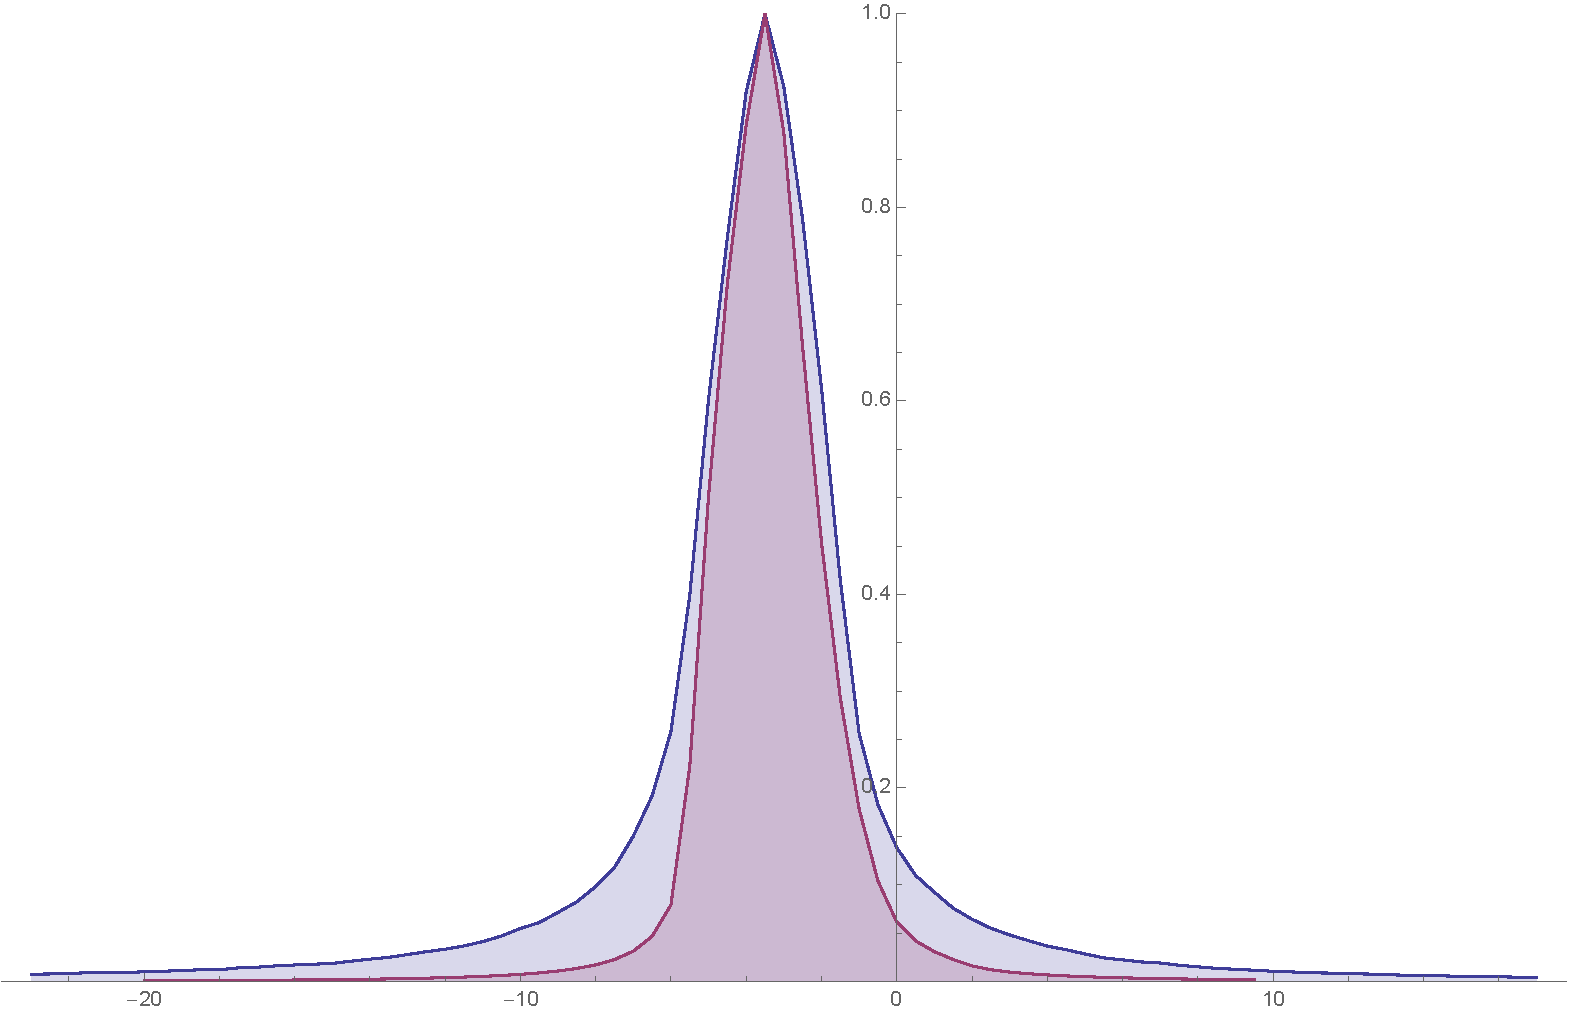
\includegraphics[width=1.5in]{img/220.eps} \\
   {$Si[220]; \theta_{B} = 10.6436$}\\

\end{minipage}\hfill
\begin{minipage}[t]{.33\textwidth}
\centering
   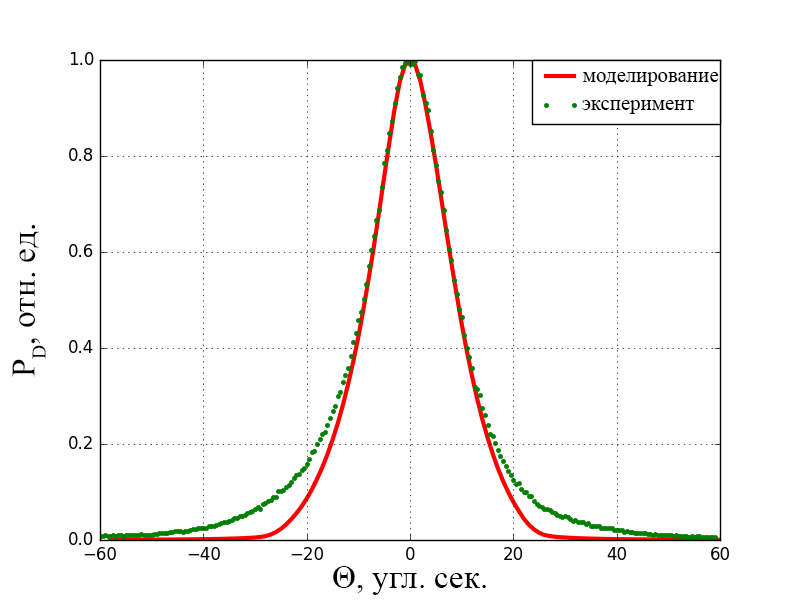
\includegraphics[width=1.5in]{img/440.eps} \\
   {$Si[440]; \theta_{B} = 21.679$}\\

\end{minipage}\hfill
\begin{minipage}[t]{.33\textwidth}
\centering
   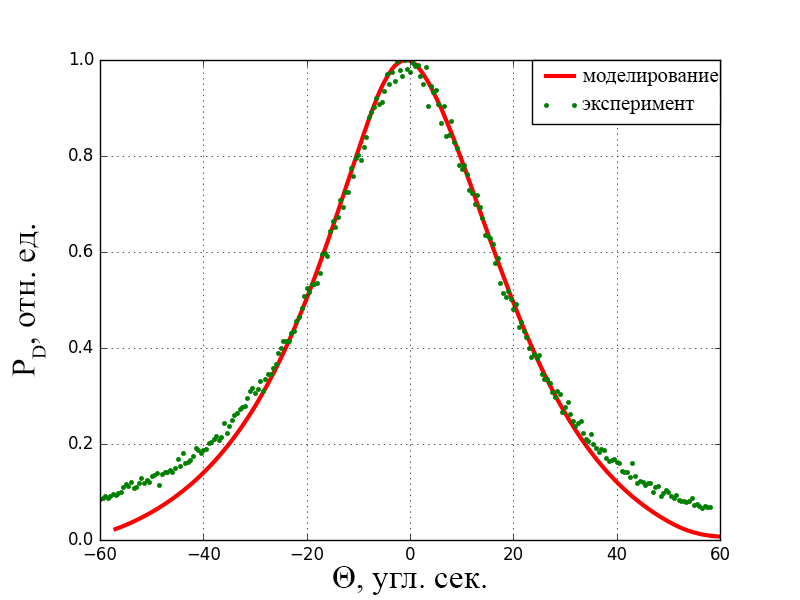
\includegraphics[width=1.5in]{img/660.eps} \\
	{$Si[660]; \theta_{B} = 33.650$} \\

\end{minipage}
\end{figure}
\end{frame}


\begin{frame}{Как влияет шаг свертки КДО}

\begin{figure}
\begin{minipage}[t]{.33\textwidth}
\centering
   \includegraphics[width=1.5in]{img/stepping/281.eps} \\
   {\scriptstyle\text{$\delta\vartheta = 1 ;(\delta\theta =    2;(\delta\eta = 8) )  $}}
\end{minipage}\hfill
\begin{minipage}[t]{.33\textwidth}
\centering
   \includegraphics[width=1.5in]{img/stepping/241.eps} \\
   {\scriptstyle\text{$\delta\vartheta = 1 ;(\delta\theta =    2;(\delta\eta = 4) )  $}}
\end{minipage}\hfill
\begin{minipage}[t]{.33\textwidth}
\centering
   \includegraphics[width=1.5in]{img/stepping/221.eps} \\
	{\scriptstyle\text{$\delta\vartheta = 1 ;(\delta\theta =    2;(\delta\eta = 2) )  $}}

\end{minipage}

\begin{minipage}[t]{.33\textwidth}
\centering
   \includegraphics[width=1.5in]{img/stepping/121.eps} \\
	{\scriptstyle\text{$\delta\vartheta = 1 ;(\delta\theta =    2;(\delta\eta = 1) )  $}}
\end{minipage}\hfill
\begin{minipage}[t]{.33\textwidth}
\centering
   \includegraphics[width=1.5in]{img/stepping/111.eps} \\
{\scriptstyle\text{$\delta\vartheta = 1 ;(\delta\theta =    1;(\delta\eta = 1) )  $}}
\end{minipage}\hfill
\begin{minipage}[t]{.33\textwidth}
\centering
   \includegraphics[width=1.5in]{img/stepping/050505.eps} \\
{\scriptstyle\text{$\delta\vartheta = 0.5 ;(\delta\theta = 0.5;(\delta\eta = 0.5) )  $}}
\end{minipage}
\end{figure}
\end{frame}



% page#5
\begin{frame}{Влияние дисперсии}
  \begin{figure}
\includegraphics[height=0.5\linewidth]{img/stepping/010105.eps}\\
{\scriptstyle\text{$\delta\vartheta = 0.5 ;(\delta\theta = 0.1;(\delta\eta = 0.1
) )  $}}
\end{figure}
\end{frame}



\end{document}


